% !TeX document-id = {63dff02d-570f-4893-a051-d8fff41185c6}
%pdflatex -shell-escape annexe1.tex
%pythontex annexe1.tex
%pdflatex -shell-escape doc5.tex
% !TeX TXS-program:compile = txs:///pdflatex/[--shell-escape]
\documentclass[12pt,french]{article}
\usepackage[utf8]{inputenc}
\usepackage[T1]{fontenc} 
\usepackage{lmodern}
\usepackage{babel}
\usepackage{xcolor}
\usepackage{minted}
\usepackage{array,multicol,multirow,enumerate,eurosym,latexsym,fourier,bbding,pifont}
\usepackage{pythontex}
\usepackage{array,multicol,multirow,enumerate,eurosym,latexsym,fourier,bbding,pifont}
\usepackage{fourier}
\usepackage{graphicx,pst-all}
\usepackage{tabularx}
\usepackage [alwaysadjust]{paralist}
\usepackage{amsmath,amsfonts,amsthm,amssymb,geometry}
\usepackage{fancyhdr}
\usepackage{mathrsfs}  
\usepackage{pstricks,pst-plot,pst-text,pst-tree,pstricks-add,pst-eps,pst-fill,pst-node,pst-math}
\usepackage{euscript,amsfonts,eepic,color}
\usepackage{ifthen,fp}
\newcommand{\Calig}[1]{\ensuremath{\mathscr{#1}}}              
\usepackage{babel}
\usepackage{xcolor}
\usepackage{minted}
\usepackage{pythontex}
\usepackage{multicol}
\usepackage[most]{tcolorbox}
\usepackage{fancyhdr}
\setlength{\parindent}{0pt}
\usepackage{ulem}
\geometry{vmargin=15mm,hmargin=5mm}
\usepackage[most]{tcolorbox}
\setlength{\parindent}{0pt}
\begin{document}

\lhead{Lycée Jean Monnet - \textit{NSI}}
\chead{}
\rhead{\textit{Année} 2019/2020}
\renewcommand{\headrulewidth}{0.5pt}
\lfoot{                      }\cfoot{Page \thepage}\rfoot{\textsf{Aude Duhem et Patrice Nicolas}}
\pagestyle{fancy}
\renewcommand{\footrulewidth}{0.4pt}
\begin{center}
	\Large{\textbf{Activités d'introduction au chapitre}}
\end{center} 
\hrule
\medskip
\large{\textbf{Activité 1 :}}\\
\normalsize
Sur la plage, un surveillant  de baignade (S) aperçoit un nageur (N) en difficulté. Le surveillant dispose d'un ordinateur qui lui "suggère" plusieurs chemins possibles pour atteindre et tenter de sauver le baigneur. \\
La Figure ci-dessus schématise la situation ; le sauveteur peut utiliser plusieurs chemins : ceux en traits pleins assurent un temps de nage minimum pour rejoindre le nageur. Le chemin en pointillés vert est celui "de moindre temps" : \textbf{c'est la solution optimale !}\\
\begin{minipage}{0.6\linewidth}
\begin{center}
	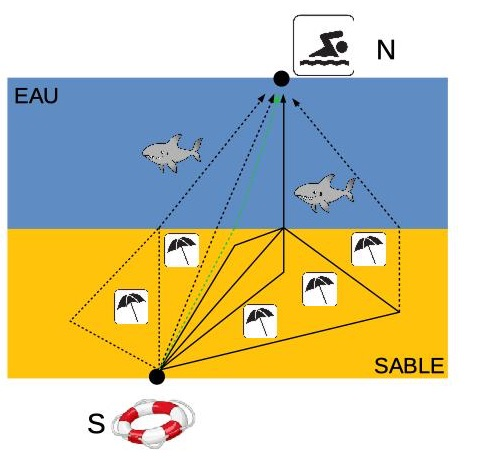
\includegraphics[scale=0.45]{Surveillant2}
\end{center}
\end{minipage}
\begin{minipage}{0.4\linewidth}
Analysons cette situation plus en détail:
\begin{itemize}
	\item Le problème est de sauver une personne.
	\item Il existe peut-être une solution pour résoudre ce problème...
	\item Si plusieurs solutions existent, on peut affirmer que la solution \textbf{"chemin de moindre temps"} fait partie de cet ensemble de solutions.
\end{itemize}
\end{minipage}
\begin{center}
	Partie A - Approche naïve
\end{center}
Le surveillant se dit:"je vais étudier  \textbf{un à un tous les chemins} puis, calculer les temps de parcours et je garderai le chemin correspondant au minimum ;  \textbf{je suis certain alors de trouver le meilleur chemin !!"}
\vspace{2mm}
\begin{enumerate}
	\item Citer un avantage et un inconvénient de la méthode proposée par le surveillant ?
	\item Quel critère pourrait-on se donner pour éliminer certains chemins ?
	\item Avec votre critère, le chemin optimal serait-il conservé ?
\end{enumerate}
\begin{center}
	Partie B - Approche "gloutonne"
\end{center}
	L'ordinateur propose le critère suivant : "Comme vous avancez moins vite dans l'eau que sur le sable, je vous propose de classer les chemins de façon à rester le moins longtemps possible dans l'eau. \textbf{ On élimine tous les autres !! C'est la méthode gloutonne, on élimine beaucoup de chemins!!} ;  les chemins conservés sont ceux représentés en traits plein sur la figure.
	\begin{enumerate}
	\item Citer un avantage et un inconvénient de la méthode proposée par l'ordinateur?
\end{enumerate}

\hrule
\medskip 
\begin{minipage}{0.75\linewidth}
\large{\textbf{Activité 2 :}}
\normalsize\\
Supposons que vous êtes un commerçant. Une cliente vous achête pour 134,34\, \euro\, de marchandise. Elle vous tend un billet de 100 \euro\, et un billet de 50 \euro.\\
Votre caisse n'est constituée que de pièces et possède autant de pièces que l'on veut. 
\begin{enumerate}
	\item Quel montant devez-vous rendre ? 
	\item Proposez au moins quatre façons différentes de rendre la monnaie.
	\item Quelle est la méthode où vous rendriez le plus de pièces possibles ?
	\item Est-ce est selon vous, la méthode employée par un caissier expérimenté ? \\
	Si non, quelle est sa méthode ? La décrire en langage naturel.
	\item Quel est le rendu proposé par votre méthode ?
\end{enumerate}
\end{minipage}
\begin{minipage}{0.25\linewidth}
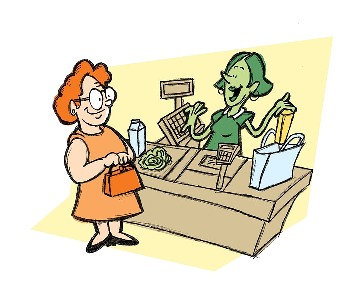
\includegraphics[scale=0.8]{caissier}\\
\begin{flushright}
	CC by Pixabay
\end{flushright}
\end{minipage}
\newpage
\textbf{Pistes de solutions pour le professeur :}\\
\textbf{Activité 1 :}\\
\begin{center}
	Partie A - Approche naïve
\end{center}
\begin{enumerate}
	\item La méthode proposée par le sauveteur assure de trouver la meilleure solution possible mais elle est très couteuse en temps !
	\item Supposons que les 9 chemins soient numérotés de gauche à droite. Quelques critères possibles:
	\begin{itemize}
		\item "Chemin(s) laissant tous les parasols à droite" :  chemins possibles \{n°1\}
		\item "Chemin(s) où le temps sur le sable est minimum" : chemins possibles \{n°2\}
		\item "Chemin(s) où le temps dans l'eau est minimum" : chemins possibles \{n°5, n°6, n°7\}
		\item ...\\
	\end{itemize}
\item Aucun des trois critères précédents ne contient la solution finale optimale. Avec ces critères, la méthode de l'ordinateur est dite sous-optimale !
\end{enumerate}
\begin{center}
	Partie B - Approche "gloutonne"
\end{center}
\begin{enumerate}
	\item La méthode gloutonne assure une certaine rapidité d'exécution mais sa réponse dépend du critère de décision choisi et en pratique elle est sous-optimale.
\end{enumerate}
\medskip
\hrule
\medskip
\textbf{Activité 2 :}\\
\begin{enumerate}
	\item on doit rendre 100\euro+50\euro-134,34\euro soit 15,66\euro.
	\item première façon : 15 pièces de 1\euro, 3 pièces de 20 centimes et 3 pièces de deux centimes soit 21 pièces\\
	deuxième façon : 7 pièces de 2 \euro, 1 pièce de 1\euro, 3 pièces de 20 centimes et 3 pièces de deux centimes soit 14 pièces\\
	troisième façon : 7 pièces de 2 \euro, 1 pièce de 1\euro, 1 pièce de 50 centimes, 1 pièce de 10 centimes et 3 pièces de deux centimes soit 13 pièces\\
	quatrième façon : 7 pièces de 2 \euro, 1 pièce de 1\euro, 6 pièces de 10 centimes et 3 pièces de deux centimes soit 17 pièces
\item La méthode avec le plus de pièces possibles est 1566 pièces de 0,01 \euro
\item Cela n'est pas la méthode du caissier expérimenté, son but est de rendre le moins de pièce possible afin d'aller au plus vite pour passer au client suivant.\\
Il est possible que deux méthodes "sortent" : l'algorithme glouton naïf et celui où on fait des divisions au lieu des soustractions.\\
(cf cours pour leur écriture).\\
leur faire écrire en pseudo code les deux afin d'introduire le cours
\item La méthode avec le moins de pièces possibles décrite ci-dessus est :\\
 7 pièces de 2 \euro, 1 pièce de 1\euro, 1 pièce de 50 centimes, 1 pièce de 10 centimes , 1 pièce de 5 centimes, 1 pièce de 1 centimes soit 12 pièces.
\end{enumerate}
\end{document}